\subsection{Possible improvements to Plotly Dash}
The main downside of using Plotly Dash is that it is not designed for real time
applications and lacks native support for . On their website they only propose
using an interval component to poll the server for updates at regular intervals
    [2]. This works, but if data should be sent from the server as soon as it becomes
available, like when you are recording video, it is not the best solution.
Another small downside is that Plotly Dash is built on top of Flask, a thread
based server framework which is slower than newer asynchronous alternatives.

\subsection{Replacing Flask backend with Quart}
The first step in the development of the \guif was to replace the Flask backend with \gls{quart}.
As the comperaison in Listing \ref{listing:concurrency_test} shows, \gls{asyncio} baseded code has significantly less overhead than asynchronous code based threads in \py.


Snehil Vijay has created a fork of \gls{dash}, called \gls{async-dash}, that replaces the Flask backend with \gls{quart} \cite{vijaySnehilvjAsyncdash2023}.
Another project aimed at making \gls{dash} run \gls{quart} called \code{dash_deviced} was also tested, but was not as easy to use as the fork by Snehil Vijay, and did not have any acivity for the last  \cite{legrandCodeFrequencyRichlegrand}.


\subsection{Adding support for websockets}
\glspl{ws} is technology that enables two-way communication between a user's browser and a server.
\cite{farhutsWebSocketsBeginnersPart2019}.
Unlike traditional HTTP, which requires the browser to request information from the server, \glspl{ws} allow for a persistent \gls{tcp} connection as visualized in Figure \ref{fig:websockets_vs_http} \cite{tingUnderstandingWebSocketsIts2020}.
This enables the server to push data to the browser when it becomes available.

Beyon this, \glspl{ws} also offer an easy way to communicate between processes similar to \gls{tcp} sockets, but with a simpler interface \cite{kanakaAnswerDifferencesTCP2013}.
\begin{figure}[H]
    \centering
    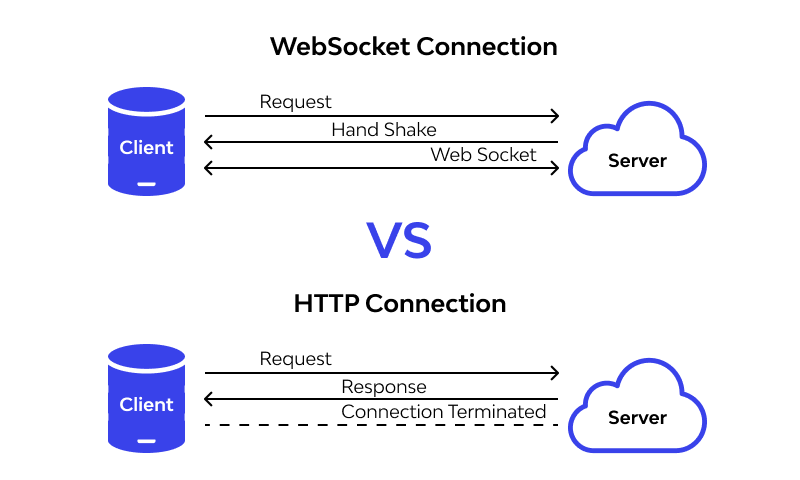
\includegraphics[width=0.8\textwidth]{figures/gui/http_vs_ws.png}
    \caption{\glspl{ws} Vs HTTP \cite{wallarmWebSocketVsHTTP}}
    \label{fig:websockets_vs_http}
\end{figure}

A significant motivation for using \gls{quart} as backend is that it supports \glspl{ws} nativly \cite{quartUsingWebsocketsQuart}.
\gls{dash} does not support \glspl{ws} out of the box, but this feature can be added through the \gls{dashextensions} library \cite{eriksenDashExtensionsWebSocket}.
Using \gls{ws} for real time updates in \gls{dash} is both a lot easier and a lot faster than the recomended way, which is to poll the server for updates at regular intervals \cite{plotlyLiveUpdatesDash}.

\subsection{Publish-subscribe framework}
\label{sec:pubsub}
To make it easier to work with \gls{ws} in \gls{dash} a small publisher-subscriber framework was developed.
This framework makes it easy to communicate between the \srgui and various processes.
It is used among other things to update the images in the \srgui, in real time, from the topics \code{"image_left"} and \code{"image_right"} which the \gls{pipeline} publishes.
It also makes it possible to send commands to the \gls{pipeline} to start and stop recordings as well as adjust camera settings.
A full set of topics is shown in Figure \ref{fig:pub_sub_graph}.

As the framwork is running as a part of the \gls{dash} server, connecting a client to it is done using the following pattern:
\begin{minted}{python}
        url = f"ws://{host}:{port}/pubsub?pub={topic_pub}&sub={topic_sub}"
        async with Connect(url) as ws:
            ...
\end{minted}
Having a client publish or subscribe to multiple topics is also possible, but not done in the \srgui.


\begin{figure}[H]
    \centering
    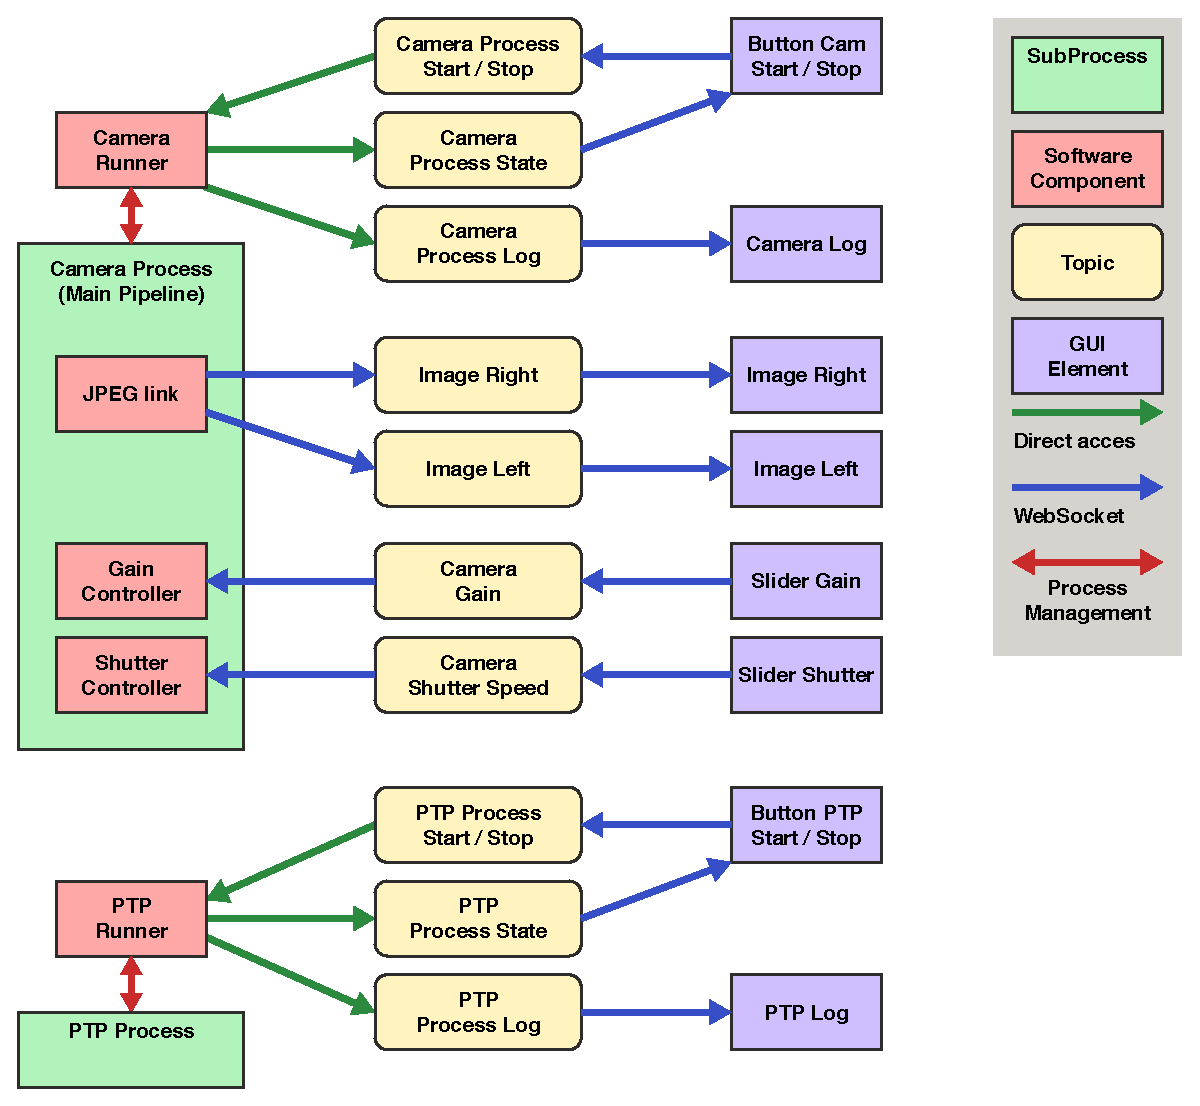
\includegraphics[width=\textwidth]{figures/gui/pubsub_graph.pdf}
    \caption{Overview of the publisher-subscriber framework.}
    \label{fig:pub_sub_graph}
\end{figure}

\subsection{Multi-page apps}
Dash supports multi-page apps, making it possible to create a web application with multiple pages that the user can navigate between \cite{plotlyMultiPageAppsURL}.
The primary intended use for this is to have separate pages on the \srgui.
One for cameara control and visualization, one for starting and monitoring recordings and one for general monitoring of the system.
A developer named Ann Marie Ward has created a set of examples on how to work with multi-page apps that was used as a starting point \cite{wardExamplesMultipageApps03Jul22}.
One major issue was that \gls{async-dash} did not work with multi-page apps.
Fortunately there is an open pull-request that fixes this issue \cite{lekAddFlaskRequest2022}.